
\documentclass[12pt, a4paper]{article}

%-----------USEPACKAGE----------------------------
\usepackage{bm} % Tucne pismo
\usepackage[czech]{babel} % Cestina
\usepackage[T1]{fontenc}
\usepackage[utf8x]{inputenc}
\linespread{1.10} % Radkovani 1.3 odpovida radkovani 2
\usepackage{lmodern} % Daji se pouzit \HUGE atd.
\usepackage{amsmath}
\usepackage{algorithm}
\usepackage[noend]{algpseudocode} % Vkladani pseudo kodu
\usepackage{listings}
\usepackage{setspace}

% Graphics
\usepackage{graphicx}
\usepackage{epstopdf}
\usepackage{color}
\graphicspath{{./img/}}

% Hyperref and its color
\usepackage[unicode]{hyperref} % Odkazy v pdf, www a na e-mail
\usepackage[hypcap=true]{caption}
\usepackage[hypcap=true,list=true]{subcaption}
\hypersetup{colorlinks = true, citecolor = black}
\hypersetup{linkcolor=red}
\hypersetup{colorlinks,urlcolor=black}





%-----------COLORS--------------------------------
\definecolor{Code}{rgb}{0,0,0}
\definecolor{Decorators}{rgb}{0.5,0.5,0.5}
\definecolor{Numbers}{rgb}{0.5,0,0}
\definecolor{MatchingBrackets}{rgb}{0.25,0.5,0.5}
\definecolor{Keywords}{rgb}{0,0,1}
\definecolor{self}{rgb}{0,0,0}
\definecolor{Strings}{rgb}{0,0.63,0}
\definecolor{Comments}{rgb}{0,0.63,1}
\definecolor{Backquotes}{rgb}{0,0,0}
\definecolor{Classname}{rgb}{0,0,0}
\definecolor{FunctionName}{rgb}{0,0,0}
\definecolor{Operators}{rgb}{0,0,0}
\definecolor{Background}{rgb}{1, 1, 1}

%-----------LISTINGS-SETTINGS----------------------
\lstset{
	numbers=left,
	numberstyle=\footnotesize,
	numbersep=0.5em,
	xleftmargin=1.5em,
	xrightmargin=0em,
	framextopmargin=0em,
	framexbottommargin=0em,
	showspaces=false,
	showtabs=false,
	showstringspaces=false,
	frame=lrtb,
	tabsize=4,
	% Basic
	basicstyle=\ttfamily\footnotesize\setstretch{1},
	backgroundcolor=\color{Background},
	language=Python,
	% Comments
	commentstyle=\color{Comments}\slshape,
	% Strings
	stringstyle=\color{Strings},
	morecomment=[s][\color{Strings}]{"""}{"""},
	morecomment=[s][\color{Strings}]{'''}{'''},
	% Keywords
morekeywords={import,from,class,def,for,while,if,is,in,elif,else,not,and,or,print,break,continue,return,True,False,None,access,as,del,except,exec,finally,global,import,lambda,pass,print,raise,try,assert},
	keywordstyle={\color{Keywords}\bfseries},
	% Additional keywords
	morekeywords={[2]@invariant},
	keywordstyle={[2]\color{Decorators}\slshape},
	emph={self},
	emphstyle={\color{self}\slshape},
	breaklines=true, % Zalamuje radky.
}






%------------------VARIABLES----------------------------
\newcommand{\cisloCviceni}{3. cvičení}









%------------------LAYOUT----------------------------
\usepackage[top = 2.5 cm, bottom = 2.5 cm, left = 2.5 cm, right = 2.5 cm]{geometry} % geometrie stranky
\usepackage{longtable}% Pro dlouhy obsah, da se zalomit \pagebrek
\usepackage{fancyhdr}
\pagestyle{fancy}% Deffaultni nastaveni hlavicky a paticky
\setlength{\headheight}{16 pt}% Zvetsi hlavicku, aby to nedelalo warningy
\fancyhf{}
\lhead{\href{http://www.kky.zcu.cz/cs/courses/mpv}{Metody Počítačového Vidění}}
\rhead{\cisloCviceni}
\fancyfoot[R]{\thepage}
\fancyfoot[L]{Verze 2.0.0, poslední úpravy: \today}








%---------------BEGIN-DOCUMENT--------------------------
\begin{document}
 









 
%--------TITLE-PAGE--------------------------------------------
\begin{titlepage}
\begin{center}
	
\includegraphics[trim = 0.6cm 0.5cm 0.9cm 0.5cm, scale=1]{./FAV_logo_cz.pdf}
	\hspace*{\fill}
	
\includegraphics[trim = 3.5cm 1.5cm 2.6cm 2cm, scale=0.295]{./KKY_logo_cz.pdf}\\
	\vspace*{\fill}
	\textbf{\Huge{\href{http://www.kky.zcu.cz/cs/courses/mpv}{Metody Počítačového Vidění} \\ ~ \\ \cisloCviceni}}\\
	\vspace*{\fill}
	\textbf{\large{\href{mailto:LBures@kky.zcu.cz}{Ing. Lukáš Bureš}}} \hfill \textbf{\large{Plzeň, \today}}
\end{center}
\end{titlepage}












%--------OBSAH-CVICENI---------------------------------
\section*{Obsah cvičení}
\begin{enumerate}
	\item Postup odevzdávání semestrálních prací
	\item Zadání 1. semestrální práce
	\item Harris Corner Detector
	\item Canny Edge Detector
\end{enumerate}







%--------ODEVZDANI-TESTOVACI-ULOHY-SKRZE-SAKO-----------------
\section{Postup odevzdávání semestrálních prací}

\begin{enumerate}
	\item Provést registraci - odkaz lze najít na stránkách \href{http://www.kky.zcu.cz/cs/courses/mpv}{MPV}.
	\item Při registraci zvolit skupinu MPV a použít email \textsf{@students.zcu.cz}.
	\item V souboru (nutno udělat u každé úlohy) \textsf{submit.py} vyplnit \textsf{login} a \textbf{tajné} heslo \textsf{passwd}.
	\item Ve složce \textsf{./src/} je vždy Python skript jehož metody je nutné implementovat.
	\item Ve složce \textsf{./src/} nesmí být žádný jiný soubor.
	\item Pro odevzdání úlohy stačí napsat do konzole: \textsf{python submit.py}
	\item Odevzdání úlohy je možné vždy v 15 minutovém intervalu.
	\item Po úspěšném odevzdání lze kontrolovat dosažené výsledky na webové stránce, kterou lze nalézt na stránkách \href{http://www.kky.zcu.cz/cs/courses/mpv}{MPV}.
\end{enumerate}






%--------ZADANI-1.-SEMESTRALNI-PRACE-------------------------
\section{Zadání 1. semestrální práce}
\par{Konkrétní zadání 1. semestrální práce je možné nalézt na internetových stránkách \href{http://www.kky.zcu.cz/cs/courses/mpv}{MPV}.}






\newpage





%--------HARRIS-CORNER-DETECTOR-------------------------------
\section{Harris Corner Detector}
\par{Předpokládejme, obrázek v odstínech šedi $I$. Dále mějme posuvné okénko $w(x, y)$ (s posunem $u$ ve směru $x$ a $v$ ve směru $y$) přes obrázek $I$. Můžeme vypočítat změnu intenzity intenzity
\begin{equation}
	E(u, v) = \sum_{x,y} w(x, y) \left[ I(x + u, y + v) - I(x, y) \right]^2,
\end{equation}
kde $w(x,y)$ je okénko na pozici $(x,y)$, $I(x,y)$ je intenzita na pozici $(x,y)$ a $I(x+u,y+v)$ je intenzita na posuvném okénku $(x+u,y+v)$.}

\par{Vzhledem k tomu, že hledáme taková okna s rohy, tedy hledáme okna s velkým rozdílem v intenzitě
\begin{equation}
	\sum_{x,y} \left[ I(x + u, y + v) - I(x, y)\right]^2,
\end{equation}
využijeme Taylorův rozvoj
\begin{equation}
	E(u, v) \approx \sum_{x,y}\left[I(x,y) + u I_x + v I_y - I(x,y)\right]^2,
\end{equation}
kde $I_x$ a $I_y$ jsou derivace v jednotlivých směrech, úpravou získáme
\begin{equation}
	E(u, v) \approx \sum_{x,y} u^2 I^2_x + 2uvI_x I_y + v^2 I_y^2.
\end{equation}
Což můžeme zapsat maticově jako
\begin{equation}
	E(u, v) \approx \left[ \begin{array}{cc} u & v
					\end{array} \right] \cdot \left( \sum_{x,y} w(x,y) 
					\left[ \begin{array}{cc}
					I_x^2 & I_x I_y\\
					I_x I_y & I_y^2 
					\end{array} \right] \right) \cdot
					\left[ \begin{array}{c}
					u\\
					v
					\end{array} \right].
\end{equation}
Označme
\begin{equation}
	M = \sum_{x,y} w(x,y) \left[ \begin{array}{cc}
									I_x^2 & I_x I_y\\
									I_x I_y & I_y^2 
								\end{array} \right],
\end{equation}
tedy naše rovnice má nyní tvar
\begin{equation}
	E (u, v) \approx \left[ \begin{array}{cc} u & v 	\end{array} \right] M \left[ \begin{array}{c} u \\ v	\end{array} \right].
\end{equation}}

\par{Skóre $R$ je vypočteno pro každé okénko, aby bylo zjištěno zda obsahuje roh
\begin{equation}
	R = det(M) - k \cdot (trace(M))^2,
\end{equation}
kde $det(M) = \lambda_1 \lambda_2$, $trace(M) = \lambda_1 + \lambda_2$ a konstanta $k$ je obvykle volena v rozmezí $0.04-0.06$. Pokud je hodnota větší, než stanovený práh, tak je bod $(x, y)$ vyhodnocen jako vrchol.}

\newpage

\par{Implementace pomocí \textit{OpenCV} je velice jednoduchá, stačí pouze zavolat metodu \href{http://docs.opencv.org/modules/imgproc/doc/feature_detection.html?highlight=cornerharris#cv2.cornerHarris}{\textit{cornerHarris}} a~následně její výstup znormovat a naprahovat.

\begin{figure}[!ht]
	\centering
	\begin{minipage}[t]{0.49\textwidth}
		%trim option's parameter order: left bottom right top
		
\includegraphics[width = \textwidth]{OriginalImg.png}
		\caption{Vstupní obrázek.}
		\label{fig:OriginalImg}
	\end{minipage}%
	\hfill
	\begin{minipage}[t]{0.49\textwidth}
		%trim option's parameter order: left bottom right top
		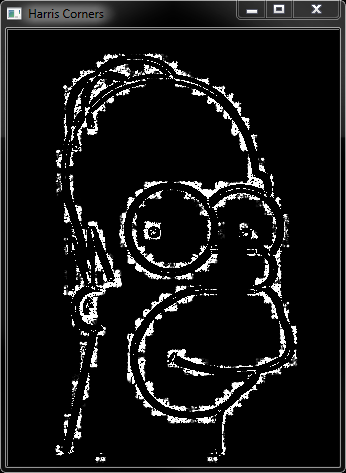
\includegraphics[width = \textwidth]{HarrisCorners.png}
		\caption{Hodnoty skóre $R$.}
		\label{fig:HarrisCorners}
	\end{minipage}%
\end{figure}
\begin{figure}[!ht]
	\centering
	\begin{minipage}[t]{0.49\textwidth}
		%trim option's parameter order: left bottom right top
		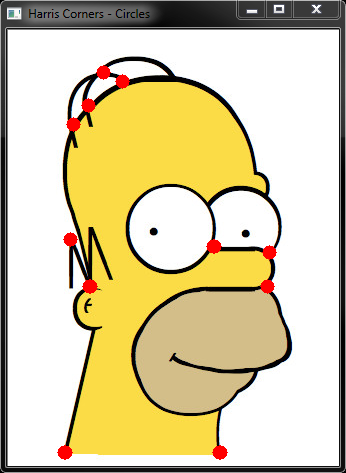
\includegraphics[width = \textwidth]{HarrisCornersCircles.png}
		\caption{Nalezené vrcholy.}
		\label{fig:HarrisCornersCircles}
	\end{minipage}%
	\hfill
	\begin{minipage}[t]{0.49\textwidth}
		%trim option's parameter order: left bottom right top
		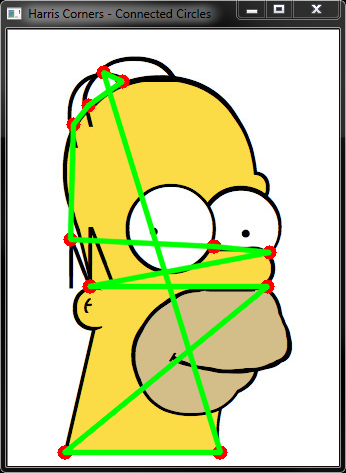
\includegraphics[width = \textwidth]{HarrisCornersConnectedCircles.png}
		\caption{Propojené vrcholy úsečkami.}
		\label{fig:HarrisCornersConnectedCircles}
	\end{minipage}%
\end{figure}


\newpage






%--------CANNY-EDGE-DETECTOR------------------------------------
\section{Canny Edge Detector}
\par{Cannyho hranový detektor je operátor detekce hran, který využívá vícestupňový algoritmus pro detekci hran v obraze. Představil ho pan John F. Canny v roce 1986, který vytvořil výpočetní teorii detekce hran s vysvětlením, proč tato technika funguje.}

\par{Cannyho detekce hran probíhá ve čtyřech krocích:
\begin{itemize}
	\item Použije se gaussovské rozmazání, aby se odstranily skvrny a šum obrazu.
	\item Aplikuje se gradientní operátor pro získání intenzit gradientů a směru.
	\item Metoda potlačení nemaxim (Non-maximum suppression - \href{http://www.kky.zcu.cz/cs/courses/mpv}{viz 1. přednáška MPV}) určí kandidáty hran.
	\item Hystereze prahování zjistí, kde hrany začínají a kde končí.		
\end{itemize}}


\newpage


\begin{figure}[!ht]
	\centering
	\begin{minipage}[t]{0.49\textwidth}
		%trim option's parameter order: left bottom right top
		
\includegraphics[width = \textwidth]{OriginalImg.png}
		\caption{Vstupní obrázek.}
		\label{fig:Homer}
	\end{minipage}%
	\hfill
	\begin{minipage}[t]{0.49\textwidth}
		%trim option's parameter order: left bottom right top
		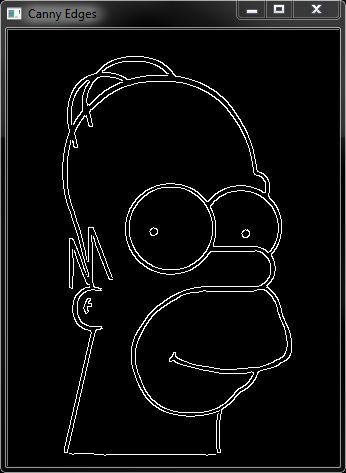
\includegraphics[width = \textwidth]{CannyHomer.png}
		\caption{Nalezené hrany.}
		\label{fig:CannyHomer}
	\end{minipage}%
\end{figure}
\begin{figure}[!ht]
	\centering
	\begin{minipage}[t]{0.49\textwidth}
		%trim option's parameter order: left bottom right top
		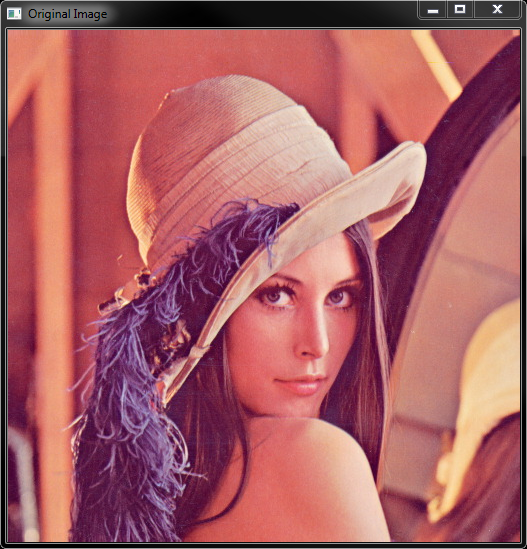
\includegraphics[width = \textwidth]{Lena.png}
		\caption{Vstupní obrázek.}
		\label{fig:Lena}
	\end{minipage}%
	\hfill
	\begin{minipage}[t]{0.49\textwidth}
		%trim option's parameter order: left bottom right top
		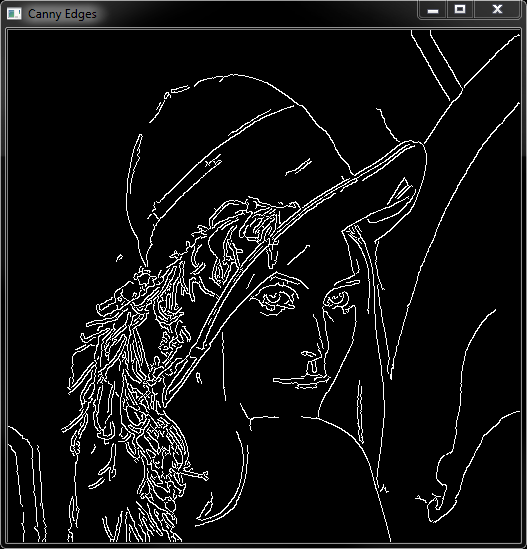
\includegraphics[width = \textwidth]{CannyLena.png}
		\caption{Nalezené hrany.}
		\label{fig:CannyLena}
	\end{minipage}%
\end{figure}












\end{document}



















